\startcontents[localtoc]
\printcontents[localtoc]{}{0}{\subsection*{Contents}\setcounter{tocdepth}{2}}

\begin{lstlisting}
% Example for algorithm ISOTS28037
\end{lstlisting}


\phantomsection
\addcontentsline{toc}{section}{Generate sample data}
\subsubsection*{Generate sample data}



Set independent and dependent variables.

\begin{lstlisting}
DI.x.v = [1 2 3 4 5];
DI.x.u = [0.1 0.1 0.1 0.1 0.1];
DI.y.v = [1.1 1.9 3.1 3.9 5.1];
DI.y.u = [0.1 0.1 0.1 0.1 0.1];

% Set values for interpolation:
DI.xhat.v = [0:0.1:6];
DI.xhat.u = 0.1 + zeros(size(DI.xhat.v));
\end{lstlisting}


\phantomsection
\addcontentsline{toc}{section}{Call algorithm}
\subsubsection*{Call algorithm}



Use QWTB to apply algorithm \texttt{ISOTS28037} to data \texttt{DI}.

\begin{lstlisting}
DO = qwtb('ISOTS28037', DI);
\end{lstlisting}
\begin{lstlisting}[language={},xleftmargin=5pt,frame=none]
QWTB: no uncertainty calculation

\end{lstlisting}


\phantomsection
\addcontentsline{toc}{section}{Display results}
\subsubsection*{Display results}



Results is

\begin{lstlisting}
disp(['offset          : ' num2str(DO.coefs.v(1)) ' +- ' num2str(DO.coefs.u(1))])
disp(['linear coeff.   : ' num2str(DO.coefs.v(2)) ' +- ' num2str(DO.coefs.u(2))])
\end{lstlisting}
\begin{lstlisting}[language={},xleftmargin=5pt,frame=none]
offset          : 1.0024 +- 0.044802
linear coeff.   : 0.012791 +- 0.14858

\end{lstlisting}


\phantomsection
\addcontentsline{toc}{section}{Plot results}
\subsubsection*{Plot results}

\begin{lstlisting}
figure
hold on
errorbar(DI.x.v, DI.y.v, DI.x.u, DI.x.u, DI.y.u, DI.y.u, '~>xb')
plot(DI.xhat.v, DO.yhat.v, 'r-')
plot(DI.xhat.v, DO.yhat.v + DI.xhat.u, 'k-')
plot(DI.xhat.v, DO.yhat.v - DI.xhat.u, 'k-')
xlabel('independent variable')
ylabel('dependent variable')
legend('original data','fit', 'interpolated values', 'uncer. of int. val.','location','southeast')
hold off
\end{lstlisting}
\begin{center}
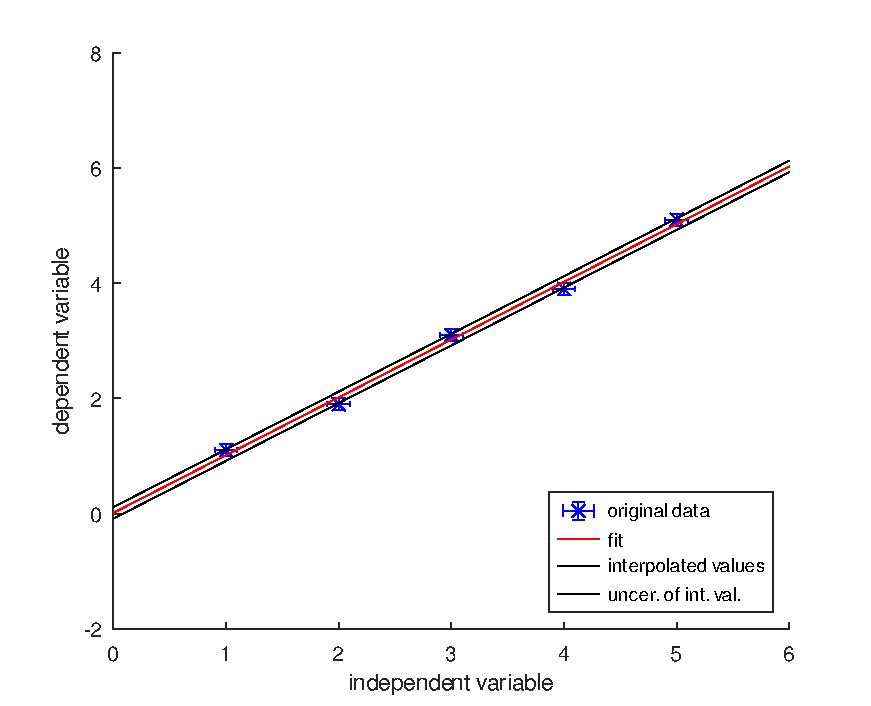
\includegraphics[width=0.7\textwidth]{algs_examples_published/ISOTS28037_alg_example-1.pdf}
\end{center}


\stopcontents[localtoc]
